\documentclass{standalone}
\usepackage{tikz}
\usetikzlibrary{positioning}
\usepackage{amsthm, amsfonts}

\begin{document}
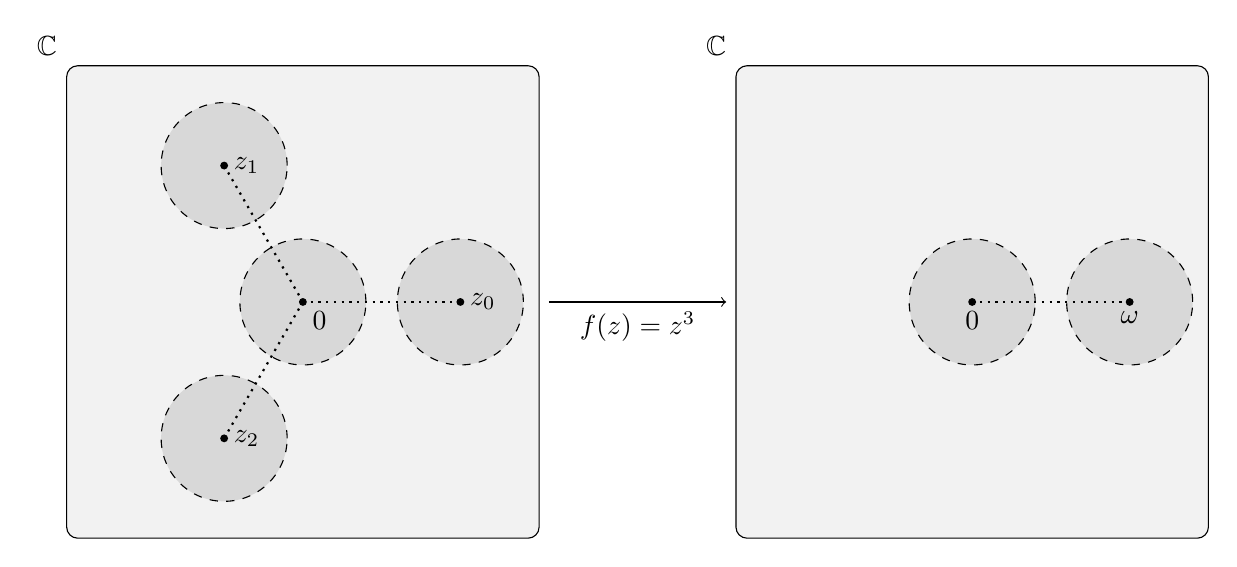
\begin{tikzpicture}
	\begin{scope}[xshift=8.5cm]
		\draw (-3,3) node[anchor=south east]{$ \mathbb{C} $};
		\filldraw[fill=gray!10, rounded corners] (-3,-3) -- (3,-3) -- (3,3) -- (-3,3) --
		cycle;
		\coordinate (cw) at (0:2);
		\coordinate (0) at (0,0);
		\filldraw[dashed, fill=gray!50, fill opacity=0.5] (0) circle[radius=0.8];
		\filldraw[dashed, fill=gray!50, fill opacity=0.5] (cw) circle[radius=0.8];
		\fill (0,0) circle[radius=.05] node[below]{$ 0 $};
		\fill (cw) circle[radius=.05] node[below]{$ \omega $};

		\draw[dotted, thick] (0) to (cw);

		\node at (-3,0) (right){};
	\end{scope}

	\coordinate (z_0) at (0:2);
	\coordinate (z_1) at (120:2);
	\coordinate (z_2) at (-120:2);

	\draw (-3,3) node[anchor=south east]{$ \mathbb{C} $};
	\filldraw[fill=gray!10, rounded corners] (-3,-3) -- (3,-3) -- (3,3) -- (-3,3) --
	cycle;
	\filldraw[dashed, fill=gray!50, fill opacity=0.5] (0,0) circle[radius=0.8];
	\fill (0,0) circle[radius=.05] node[below right]{$ 0 $};

	\foreach \p in {z_0, z_1, z_2}{
			\filldraw[dashed, fill=gray!50, fill opacity=0.5] (\p) circle[radius=0.8];
			\fill (\p) circle[radius=.05] node[right]{$ \p $};
			\draw[dotted, thick] (0,0) to (\p);
		}

	\node at (3,0) (left){};

	\draw[->] (left) to node[below]{$ f(z)=z^3 $} (right);

\end{tikzpicture}
\end{document}
